% Created by tikzDevice version 0.12.3.2 on 2022-02-15 11:53:51
% !TEX encoding = UTF-8 Unicode
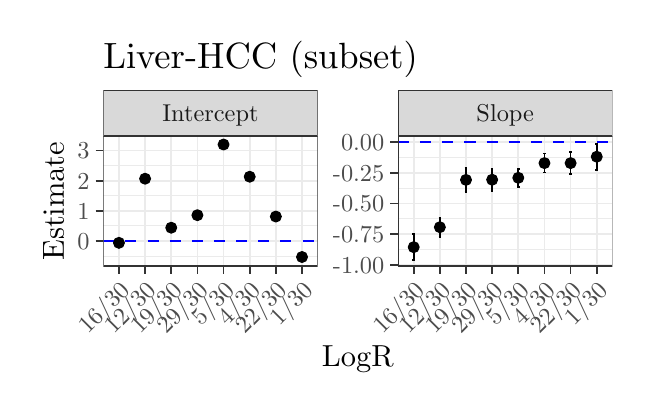
\begin{tikzpicture}[x=1pt,y=1pt]
\definecolor{fillColor}{RGB}{255,255,255}
\path[use as bounding box,fill=fillColor,fill opacity=0.00] (0,0) rectangle (216.81,130.09);
\begin{scope}
\path[clip] (  0.00,  0.00) rectangle (216.81,130.09);
\definecolor{drawColor}{RGB}{255,255,255}
\definecolor{fillColor}{RGB}{255,255,255}

\path[draw=drawColor,line width= 0.6pt,line join=round,line cap=round,fill=fillColor] (  0.00,  0.00) rectangle (216.81,130.09);
\end{scope}
\begin{scope}
\path[clip] ( 27.31, 43.96) rectangle (104.80, 90.86);
\definecolor{fillColor}{RGB}{255,255,255}

\path[fill=fillColor] ( 27.31, 43.96) rectangle (104.80, 90.86);
\definecolor{drawColor}{gray}{0.92}

\path[draw=drawColor,line width= 0.3pt,line join=round] ( 27.31, 47.58) --
	(104.80, 47.58);

\path[draw=drawColor,line width= 0.3pt,line join=round] ( 27.31, 58.46) --
	(104.80, 58.46);

\path[draw=drawColor,line width= 0.3pt,line join=round] ( 27.31, 69.35) --
	(104.80, 69.35);

\path[draw=drawColor,line width= 0.3pt,line join=round] ( 27.31, 80.23) --
	(104.80, 80.23);

\path[draw=drawColor,line width= 0.6pt,line join=round] ( 27.31, 53.02) --
	(104.80, 53.02);

\path[draw=drawColor,line width= 0.6pt,line join=round] ( 27.31, 63.90) --
	(104.80, 63.90);

\path[draw=drawColor,line width= 0.6pt,line join=round] ( 27.31, 74.79) --
	(104.80, 74.79);

\path[draw=drawColor,line width= 0.6pt,line join=round] ( 27.31, 85.67) --
	(104.80, 85.67);

\path[draw=drawColor,line width= 0.6pt,line join=round] ( 32.98, 43.96) --
	( 32.98, 90.86);

\path[draw=drawColor,line width= 0.6pt,line join=round] ( 42.43, 43.96) --
	( 42.43, 90.86);

\path[draw=drawColor,line width= 0.6pt,line join=round] ( 51.88, 43.96) --
	( 51.88, 90.86);

\path[draw=drawColor,line width= 0.6pt,line join=round] ( 61.33, 43.96) --
	( 61.33, 90.86);

\path[draw=drawColor,line width= 0.6pt,line join=round] ( 70.78, 43.96) --
	( 70.78, 90.86);

\path[draw=drawColor,line width= 0.6pt,line join=round] ( 80.23, 43.96) --
	( 80.23, 90.86);

\path[draw=drawColor,line width= 0.6pt,line join=round] ( 89.68, 43.96) --
	( 89.68, 90.86);

\path[draw=drawColor,line width= 0.6pt,line join=round] ( 99.13, 43.96) --
	( 99.13, 90.86);
\definecolor{drawColor}{RGB}{0,0,255}

\path[draw=drawColor,line width= 0.6pt,dash pattern=on 4pt off 4pt ,line join=round] ( 27.31, 53.02) -- (104.80, 53.02);
\definecolor{drawColor}{RGB}{0,0,0}
\definecolor{fillColor}{RGB}{0,0,0}

\path[draw=drawColor,line width= 0.4pt,line join=round,line cap=round,fill=fillColor] ( 99.13, 47.22) circle (  1.96);

\path[draw=drawColor,line width= 0.4pt,line join=round,line cap=round,fill=fillColor] ( 80.23, 76.23) circle (  1.96);

\path[draw=drawColor,line width= 0.4pt,line join=round,line cap=round,fill=fillColor] ( 70.78, 87.87) circle (  1.96);

\path[draw=drawColor,line width= 0.4pt,line join=round,line cap=round,fill=fillColor] ( 42.43, 75.51) circle (  1.96);

\path[draw=drawColor,line width= 0.4pt,line join=round,line cap=round,fill=fillColor] ( 32.98, 52.34) circle (  1.96);

\path[draw=drawColor,line width= 0.4pt,line join=round,line cap=round,fill=fillColor] ( 51.88, 57.81) circle (  1.96);

\path[draw=drawColor,line width= 0.4pt,line join=round,line cap=round,fill=fillColor] ( 89.68, 61.84) circle (  1.96);

\path[draw=drawColor,line width= 0.4pt,line join=round,line cap=round,fill=fillColor] ( 61.33, 62.33) circle (  1.96);

\path[draw=drawColor,line width= 0.6pt,line join=round] ( 98.66, 48.35) --
	( 99.60, 48.35);

\path[draw=drawColor,line width= 0.6pt,line join=round] ( 99.13, 48.35) --
	( 99.13, 46.09);

\path[draw=drawColor,line width= 0.6pt,line join=round] ( 98.66, 46.09) --
	( 99.60, 46.09);

\path[draw=drawColor,line width= 0.6pt,line join=round] ( 79.76, 77.09) --
	( 80.70, 77.09);

\path[draw=drawColor,line width= 0.6pt,line join=round] ( 80.23, 77.09) --
	( 80.23, 75.37);

\path[draw=drawColor,line width= 0.6pt,line join=round] ( 79.76, 75.37) --
	( 80.70, 75.37);

\path[draw=drawColor,line width= 0.6pt,line join=round] ( 70.31, 88.73) --
	( 71.25, 88.73);

\path[draw=drawColor,line width= 0.6pt,line join=round] ( 70.78, 88.73) --
	( 70.78, 87.01);

\path[draw=drawColor,line width= 0.6pt,line join=round] ( 70.31, 87.01) --
	( 71.25, 87.01);

\path[draw=drawColor,line width= 0.6pt,line join=round] ( 41.96, 76.69) --
	( 42.91, 76.69);

\path[draw=drawColor,line width= 0.6pt,line join=round] ( 42.43, 76.69) --
	( 42.43, 74.33);

\path[draw=drawColor,line width= 0.6pt,line join=round] ( 41.96, 74.33) --
	( 42.91, 74.33);

\path[draw=drawColor,line width= 0.6pt,line join=round] ( 32.51, 54.08) --
	( 33.46, 54.08);

\path[draw=drawColor,line width= 0.6pt,line join=round] ( 32.98, 54.08) --
	( 32.98, 50.60);

\path[draw=drawColor,line width= 0.6pt,line join=round] ( 32.51, 50.60) --
	( 33.46, 50.60);

\path[draw=drawColor,line width= 0.6pt,line join=round] ( 51.41, 58.81) --
	( 52.35, 58.81);

\path[draw=drawColor,line width= 0.6pt,line join=round] ( 51.88, 58.81) --
	( 51.88, 56.81);

\path[draw=drawColor,line width= 0.6pt,line join=round] ( 51.41, 56.81) --
	( 52.35, 56.81);

\path[draw=drawColor,line width= 0.6pt,line join=round] ( 89.21, 62.86) --
	( 90.15, 62.86);

\path[draw=drawColor,line width= 0.6pt,line join=round] ( 89.68, 62.86) --
	( 89.68, 60.82);

\path[draw=drawColor,line width= 0.6pt,line join=round] ( 89.21, 60.82) --
	( 90.15, 60.82);

\path[draw=drawColor,line width= 0.6pt,line join=round] ( 60.86, 63.18) --
	( 61.80, 63.18);

\path[draw=drawColor,line width= 0.6pt,line join=round] ( 61.33, 63.18) --
	( 61.33, 61.47);

\path[draw=drawColor,line width= 0.6pt,line join=round] ( 60.86, 61.47) --
	( 61.80, 61.47);
\definecolor{drawColor}{gray}{0.20}

\path[draw=drawColor,line width= 0.6pt,line join=round,line cap=round] ( 27.31, 43.96) rectangle (104.80, 90.86);
\end{scope}
\begin{scope}
\path[clip] (133.82, 43.96) rectangle (211.31, 90.86);
\definecolor{fillColor}{RGB}{255,255,255}

\path[fill=fillColor] (133.82, 43.96) rectangle (211.31, 90.86);
\definecolor{drawColor}{gray}{0.92}

\path[draw=drawColor,line width= 0.3pt,line join=round] (133.82, 49.96) --
	(211.31, 49.96);

\path[draw=drawColor,line width= 0.3pt,line join=round] (133.82, 61.04) --
	(211.31, 61.04);

\path[draw=drawColor,line width= 0.3pt,line join=round] (133.82, 72.11) --
	(211.31, 72.11);

\path[draw=drawColor,line width= 0.3pt,line join=round] (133.82, 83.19) --
	(211.31, 83.19);

\path[draw=drawColor,line width= 0.6pt,line join=round] (133.82, 44.42) --
	(211.31, 44.42);

\path[draw=drawColor,line width= 0.6pt,line join=round] (133.82, 55.50) --
	(211.31, 55.50);

\path[draw=drawColor,line width= 0.6pt,line join=round] (133.82, 66.57) --
	(211.31, 66.57);

\path[draw=drawColor,line width= 0.6pt,line join=round] (133.82, 77.65) --
	(211.31, 77.65);

\path[draw=drawColor,line width= 0.6pt,line join=round] (133.82, 88.73) --
	(211.31, 88.73);

\path[draw=drawColor,line width= 0.6pt,line join=round] (139.49, 43.96) --
	(139.49, 90.86);

\path[draw=drawColor,line width= 0.6pt,line join=round] (148.94, 43.96) --
	(148.94, 90.86);

\path[draw=drawColor,line width= 0.6pt,line join=round] (158.39, 43.96) --
	(158.39, 90.86);

\path[draw=drawColor,line width= 0.6pt,line join=round] (167.84, 43.96) --
	(167.84, 90.86);

\path[draw=drawColor,line width= 0.6pt,line join=round] (177.29, 43.96) --
	(177.29, 90.86);

\path[draw=drawColor,line width= 0.6pt,line join=round] (186.74, 43.96) --
	(186.74, 90.86);

\path[draw=drawColor,line width= 0.6pt,line join=round] (196.19, 43.96) --
	(196.19, 90.86);

\path[draw=drawColor,line width= 0.6pt,line join=round] (205.64, 43.96) --
	(205.64, 90.86);
\definecolor{drawColor}{RGB}{0,0,255}

\path[draw=drawColor,line width= 0.6pt,dash pattern=on 4pt off 4pt ,line join=round] (133.82, 88.73) -- (211.31, 88.73);
\definecolor{drawColor}{RGB}{0,0,0}
\definecolor{fillColor}{RGB}{0,0,0}

\path[draw=drawColor,line width= 0.4pt,line join=round,line cap=round,fill=fillColor] (205.64, 83.46) circle (  1.96);

\path[draw=drawColor,line width= 0.4pt,line join=round,line cap=round,fill=fillColor] (186.74, 81.15) circle (  1.96);

\path[draw=drawColor,line width= 0.4pt,line join=round,line cap=round,fill=fillColor] (177.29, 75.84) circle (  1.96);

\path[draw=drawColor,line width= 0.4pt,line join=round,line cap=round,fill=fillColor] (148.94, 57.99) circle (  1.96);

\path[draw=drawColor,line width= 0.4pt,line join=round,line cap=round,fill=fillColor] (139.49, 50.78) circle (  1.96);

\path[draw=drawColor,line width= 0.4pt,line join=round,line cap=round,fill=fillColor] (158.39, 75.09) circle (  1.96);

\path[draw=drawColor,line width= 0.4pt,line join=round,line cap=round,fill=fillColor] (196.19, 81.15) circle (  1.96);

\path[draw=drawColor,line width= 0.4pt,line join=round,line cap=round,fill=fillColor] (167.84, 75.15) circle (  1.96);

\path[draw=drawColor,line width= 0.6pt,line join=round] (205.17, 88.17) --
	(206.11, 88.17);

\path[draw=drawColor,line width= 0.6pt,line join=round] (205.64, 88.17) --
	(205.64, 78.75);

\path[draw=drawColor,line width= 0.6pt,line join=round] (205.17, 78.75) --
	(206.11, 78.75);

\path[draw=drawColor,line width= 0.6pt,line join=round] (186.27, 84.57) --
	(187.21, 84.57);

\path[draw=drawColor,line width= 0.6pt,line join=round] (186.74, 84.57) --
	(186.74, 77.73);

\path[draw=drawColor,line width= 0.6pt,line join=round] (186.27, 77.73) --
	(187.21, 77.73);

\path[draw=drawColor,line width= 0.6pt,line join=round] (176.82, 79.10) --
	(177.76, 79.10);

\path[draw=drawColor,line width= 0.6pt,line join=round] (177.29, 79.10) --
	(177.29, 72.59);

\path[draw=drawColor,line width= 0.6pt,line join=round] (176.82, 72.59) --
	(177.76, 72.59);

\path[draw=drawColor,line width= 0.6pt,line join=round] (148.47, 61.48) --
	(149.42, 61.48);

\path[draw=drawColor,line width= 0.6pt,line join=round] (148.94, 61.48) --
	(148.94, 54.50);

\path[draw=drawColor,line width= 0.6pt,line join=round] (148.47, 54.50) --
	(149.42, 54.50);

\path[draw=drawColor,line width= 0.6pt,line join=round] (139.02, 55.47) --
	(139.97, 55.47);

\path[draw=drawColor,line width= 0.6pt,line join=round] (139.49, 55.47) --
	(139.49, 46.09);

\path[draw=drawColor,line width= 0.6pt,line join=round] (139.02, 46.09) --
	(139.97, 46.09);

\path[draw=drawColor,line width= 0.6pt,line join=round] (157.92, 79.36) --
	(158.86, 79.36);

\path[draw=drawColor,line width= 0.6pt,line join=round] (158.39, 79.36) --
	(158.39, 70.81);

\path[draw=drawColor,line width= 0.6pt,line join=round] (157.92, 70.81) --
	(158.86, 70.81);

\path[draw=drawColor,line width= 0.6pt,line join=round] (195.72, 85.10) --
	(196.66, 85.10);

\path[draw=drawColor,line width= 0.6pt,line join=round] (196.19, 85.10) --
	(196.19, 77.21);

\path[draw=drawColor,line width= 0.6pt,line join=round] (195.72, 77.21) --
	(196.66, 77.21);

\path[draw=drawColor,line width= 0.6pt,line join=round] (167.37, 79.19) --
	(168.31, 79.19);

\path[draw=drawColor,line width= 0.6pt,line join=round] (167.84, 79.19) --
	(167.84, 71.12);

\path[draw=drawColor,line width= 0.6pt,line join=round] (167.37, 71.12) --
	(168.31, 71.12);
\definecolor{drawColor}{gray}{0.20}

\path[draw=drawColor,line width= 0.6pt,line join=round,line cap=round] (133.82, 43.96) rectangle (211.31, 90.86);
\end{scope}
\begin{scope}
\path[clip] ( 27.31, 90.86) rectangle (104.80,107.43);
\definecolor{drawColor}{gray}{0.20}
\definecolor{fillColor}{gray}{0.85}

\path[draw=drawColor,line width= 0.6pt,line join=round,line cap=round,fill=fillColor] ( 27.31, 90.86) rectangle (104.80,107.43);
\definecolor{drawColor}{gray}{0.10}

\node[text=drawColor,anchor=base,inner sep=0pt, outer sep=0pt, scale=  0.88] at ( 66.06, 96.11) {Intercept};
\end{scope}
\begin{scope}
\path[clip] (133.82, 90.86) rectangle (211.31,107.43);
\definecolor{drawColor}{gray}{0.20}
\definecolor{fillColor}{gray}{0.85}

\path[draw=drawColor,line width= 0.6pt,line join=round,line cap=round,fill=fillColor] (133.82, 90.86) rectangle (211.31,107.43);
\definecolor{drawColor}{gray}{0.10}

\node[text=drawColor,anchor=base,inner sep=0pt, outer sep=0pt, scale=  0.88] at (172.57, 96.11) {Slope};
\end{scope}
\begin{scope}
\path[clip] (  0.00,  0.00) rectangle (216.81,130.09);
\definecolor{drawColor}{gray}{0.20}

\path[draw=drawColor,line width= 0.6pt,line join=round] ( 32.98, 41.21) --
	( 32.98, 43.96);

\path[draw=drawColor,line width= 0.6pt,line join=round] ( 42.43, 41.21) --
	( 42.43, 43.96);

\path[draw=drawColor,line width= 0.6pt,line join=round] ( 51.88, 41.21) --
	( 51.88, 43.96);

\path[draw=drawColor,line width= 0.6pt,line join=round] ( 61.33, 41.21) --
	( 61.33, 43.96);

\path[draw=drawColor,line width= 0.6pt,line join=round] ( 70.78, 41.21) --
	( 70.78, 43.96);

\path[draw=drawColor,line width= 0.6pt,line join=round] ( 80.23, 41.21) --
	( 80.23, 43.96);

\path[draw=drawColor,line width= 0.6pt,line join=round] ( 89.68, 41.21) --
	( 89.68, 43.96);

\path[draw=drawColor,line width= 0.6pt,line join=round] ( 99.13, 41.21) --
	( 99.13, 43.96);
\end{scope}
\begin{scope}
\path[clip] (  0.00,  0.00) rectangle (216.81,130.09);
\definecolor{drawColor}{gray}{0.30}

\node[text=drawColor,rotate= 45.00,anchor=base east,inner sep=0pt, outer sep=0pt, scale=  0.88] at ( 37.27, 34.73) {16/30};

\node[text=drawColor,rotate= 45.00,anchor=base east,inner sep=0pt, outer sep=0pt, scale=  0.88] at ( 46.72, 34.73) {12/30};

\node[text=drawColor,rotate= 45.00,anchor=base east,inner sep=0pt, outer sep=0pt, scale=  0.88] at ( 56.17, 34.73) {19/30};

\node[text=drawColor,rotate= 45.00,anchor=base east,inner sep=0pt, outer sep=0pt, scale=  0.88] at ( 65.62, 34.73) {29/30};

\node[text=drawColor,rotate= 45.00,anchor=base east,inner sep=0pt, outer sep=0pt, scale=  0.88] at ( 75.07, 34.73) {5/30};

\node[text=drawColor,rotate= 45.00,anchor=base east,inner sep=0pt, outer sep=0pt, scale=  0.88] at ( 84.52, 34.73) {4/30};

\node[text=drawColor,rotate= 45.00,anchor=base east,inner sep=0pt, outer sep=0pt, scale=  0.88] at ( 93.97, 34.73) {22/30};

\node[text=drawColor,rotate= 45.00,anchor=base east,inner sep=0pt, outer sep=0pt, scale=  0.88] at (103.42, 34.73) {1/30};
\end{scope}
\begin{scope}
\path[clip] (  0.00,  0.00) rectangle (216.81,130.09);
\definecolor{drawColor}{gray}{0.20}

\path[draw=drawColor,line width= 0.6pt,line join=round] (139.49, 41.21) --
	(139.49, 43.96);

\path[draw=drawColor,line width= 0.6pt,line join=round] (148.94, 41.21) --
	(148.94, 43.96);

\path[draw=drawColor,line width= 0.6pt,line join=round] (158.39, 41.21) --
	(158.39, 43.96);

\path[draw=drawColor,line width= 0.6pt,line join=round] (167.84, 41.21) --
	(167.84, 43.96);

\path[draw=drawColor,line width= 0.6pt,line join=round] (177.29, 41.21) --
	(177.29, 43.96);

\path[draw=drawColor,line width= 0.6pt,line join=round] (186.74, 41.21) --
	(186.74, 43.96);

\path[draw=drawColor,line width= 0.6pt,line join=round] (196.19, 41.21) --
	(196.19, 43.96);

\path[draw=drawColor,line width= 0.6pt,line join=round] (205.64, 41.21) --
	(205.64, 43.96);
\end{scope}
\begin{scope}
\path[clip] (  0.00,  0.00) rectangle (216.81,130.09);
\definecolor{drawColor}{gray}{0.30}

\node[text=drawColor,rotate= 45.00,anchor=base east,inner sep=0pt, outer sep=0pt, scale=  0.88] at (143.78, 34.73) {16/30};

\node[text=drawColor,rotate= 45.00,anchor=base east,inner sep=0pt, outer sep=0pt, scale=  0.88] at (153.23, 34.73) {12/30};

\node[text=drawColor,rotate= 45.00,anchor=base east,inner sep=0pt, outer sep=0pt, scale=  0.88] at (162.68, 34.73) {19/30};

\node[text=drawColor,rotate= 45.00,anchor=base east,inner sep=0pt, outer sep=0pt, scale=  0.88] at (172.13, 34.73) {29/30};

\node[text=drawColor,rotate= 45.00,anchor=base east,inner sep=0pt, outer sep=0pt, scale=  0.88] at (181.58, 34.73) {5/30};

\node[text=drawColor,rotate= 45.00,anchor=base east,inner sep=0pt, outer sep=0pt, scale=  0.88] at (191.03, 34.73) {4/30};

\node[text=drawColor,rotate= 45.00,anchor=base east,inner sep=0pt, outer sep=0pt, scale=  0.88] at (200.48, 34.73) {22/30};

\node[text=drawColor,rotate= 45.00,anchor=base east,inner sep=0pt, outer sep=0pt, scale=  0.88] at (209.93, 34.73) {1/30};
\end{scope}
\begin{scope}
\path[clip] (  0.00,  0.00) rectangle (216.81,130.09);
\definecolor{drawColor}{gray}{0.30}

\node[text=drawColor,anchor=base east,inner sep=0pt, outer sep=0pt, scale=  0.88] at (128.87, 41.39) {-1.00};

\node[text=drawColor,anchor=base east,inner sep=0pt, outer sep=0pt, scale=  0.88] at (128.87, 52.47) {-0.75};

\node[text=drawColor,anchor=base east,inner sep=0pt, outer sep=0pt, scale=  0.88] at (128.87, 63.54) {-0.50};

\node[text=drawColor,anchor=base east,inner sep=0pt, outer sep=0pt, scale=  0.88] at (128.87, 74.62) {-0.25};

\node[text=drawColor,anchor=base east,inner sep=0pt, outer sep=0pt, scale=  0.88] at (128.87, 85.70) {0.00};
\end{scope}
\begin{scope}
\path[clip] (  0.00,  0.00) rectangle (216.81,130.09);
\definecolor{drawColor}{gray}{0.20}

\path[draw=drawColor,line width= 0.6pt,line join=round] (131.07, 44.42) --
	(133.82, 44.42);

\path[draw=drawColor,line width= 0.6pt,line join=round] (131.07, 55.50) --
	(133.82, 55.50);

\path[draw=drawColor,line width= 0.6pt,line join=round] (131.07, 66.57) --
	(133.82, 66.57);

\path[draw=drawColor,line width= 0.6pt,line join=round] (131.07, 77.65) --
	(133.82, 77.65);

\path[draw=drawColor,line width= 0.6pt,line join=round] (131.07, 88.73) --
	(133.82, 88.73);
\end{scope}
\begin{scope}
\path[clip] (  0.00,  0.00) rectangle (216.81,130.09);
\definecolor{drawColor}{gray}{0.30}

\node[text=drawColor,anchor=base east,inner sep=0pt, outer sep=0pt, scale=  0.88] at ( 22.36, 49.99) {0};

\node[text=drawColor,anchor=base east,inner sep=0pt, outer sep=0pt, scale=  0.88] at ( 22.36, 60.87) {1};

\node[text=drawColor,anchor=base east,inner sep=0pt, outer sep=0pt, scale=  0.88] at ( 22.36, 71.76) {2};

\node[text=drawColor,anchor=base east,inner sep=0pt, outer sep=0pt, scale=  0.88] at ( 22.36, 82.64) {3};
\end{scope}
\begin{scope}
\path[clip] (  0.00,  0.00) rectangle (216.81,130.09);
\definecolor{drawColor}{gray}{0.20}

\path[draw=drawColor,line width= 0.6pt,line join=round] ( 24.56, 53.02) --
	( 27.31, 53.02);

\path[draw=drawColor,line width= 0.6pt,line join=round] ( 24.56, 63.90) --
	( 27.31, 63.90);

\path[draw=drawColor,line width= 0.6pt,line join=round] ( 24.56, 74.79) --
	( 27.31, 74.79);

\path[draw=drawColor,line width= 0.6pt,line join=round] ( 24.56, 85.67) --
	( 27.31, 85.67);
\end{scope}
\begin{scope}
\path[clip] (  0.00,  0.00) rectangle (216.81,130.09);
\definecolor{drawColor}{RGB}{0,0,0}

\node[text=drawColor,anchor=base,inner sep=0pt, outer sep=0pt, scale=  1.10] at (119.31,  7.64) {LogR};
\end{scope}
\begin{scope}
\path[clip] (  0.00,  0.00) rectangle (216.81,130.09);
\definecolor{drawColor}{RGB}{0,0,0}

\node[text=drawColor,rotate= 90.00,anchor=base,inner sep=0pt, outer sep=0pt, scale=  1.10] at ( 13.08, 67.41) {Estimate};
\end{scope}
\begin{scope}
\path[clip] (  0.00,  0.00) rectangle (216.81,130.09);
\definecolor{drawColor}{RGB}{0,0,0}

\node[text=drawColor,anchor=base west,inner sep=0pt, outer sep=0pt, scale=  1.32] at ( 27.31,115.49) {Liver-HCC (subset)};
\end{scope}
\end{tikzpicture}
